\section{\textit{Logistic Regression}}
\label{sec:lr}

\todo{Satu paragraf pengantar: peran LR dalam tugas ini dan ringkasan hasil terbaiknya.}

\subsection{Implementasi \textit{From Scratch}}
\label{subsec:lr-implementasi}

\subsubsection{Landasan Teori}

\paragraph{Model.} Untuk vektor fitur $x \in \mathbb{R}^d$, LR memodelkan peluang kelas positif (batal) sebagai
\begin{equation}
	p = P(y = 1 \mid x) = \sigma(w \cdot x + b), \qquad \sigma(z) = \frac{1}{1 + e^{-z}},
	\label{eq:lr-model}
\end{equation}
dengan bobot $w$ dan bias $b$. Fungsi sigmoid memetakan skor linear ke rentang $(0, 1)$, sehingga keluaran LR adalah \textit{soft classification}. Label diperoleh dengan aturan $\hat{y} = 1$ jika $p \ge t$; materi kelas memakai $t = 0{,}5$ \cite{khodra-lr-what,khodra-lr-sga}, sedangkan pada tugas ini $t$ dipilih lewat validasi silang (Subbab~\ref{subsec:lr-validasi}).

\paragraph{Fungsi \textit{loss}.} Parameter dicari dengan \textit{maximum likelihood estimation}, yaitu memaksimumkan \textit{log conditional likelihood} (LCL) $\sum_i [\,y_i \log p_i + (1-y_i)\log(1-p_i)\,]$ \cite{khodra-lr-sga}. Implementasi meminimumkan bentuk yang setara, yaitu rata-rata \textit{log-loss} ditambah penalti regularisasi:
\begin{equation}
	J(w, b) = -\frac{1}{n}\sum_{i=1}^{n} c_i\big[\,y_i \log p_i + (1-y_i)\log(1-p_i)\,\big] + \lambda\,\Omega(w),
	\label{eq:lr-loss}
\end{equation}
dengan $c_i$ bobot sampel (bernilai 1 kecuali pada \textit{cost-sensitive learning}, Subbab~\ref{sec:cost-sensitive}) dan $\lambda \ge 0$ kekuatan regularisasi. Gradien suku \textit{log-loss} terhadap $w$ adalah $\frac{1}{n}\sum_i c_i(p_i - y_i)\,x_i$, yaitu negatif dari turunan LCL $\sum_i (y_i - p_i)\,x_{ij}$ pada materi kelas dibagi $n$. Karena itu meminimumkan $J$ dengan \textit{gradient descent} identik dengan \textit{gradient ascent} pada LCL.

\paragraph{Regularisasi.} Penalti $\Omega(w)$ dan gradiennya ditunjukkan pada Tabel~\ref{tab:lr-penalti}. Bias $b$ tidak diregularisasi. L2 (\textit{ridge}) mengecilkan semua bobot secara halus. L1 (\textit{lasso}) mendorong sebagian bobot menjadi tepat nol sehingga sekaligus berfungsi sebagai seleksi fitur \cite{tibshirani1996lasso}. \textit{Elastic Net} menggabungkan keduanya dengan rasio $\rho$; kombinasi ini lebih stabil daripada L1 murni ketika fitur saling berkorelasi \cite{zou2005elasticnet}. Formulasi ini mengikuti \textit{scikit-learn} \cite{sklearn-lr-guide}.

\begin{table}[H]
	\centering
	\caption{Penalti regularisasi dan gradiennya}
	\label{tab:lr-penalti}
	\begin{tabular}{l c c}
		\toprule
		\textbf{\texttt{penalty}} & $\Omega(w)$ & $\nabla_w \Omega(w)$ \\
		\midrule
		\texttt{None} & $0$ & $0$ \\
		\texttt{"l2"} & $\tfrac{1}{2}\lVert w\rVert_2^2$ & $w$ \\
		\texttt{"l1"} & $\lVert w\rVert_1$ & $\operatorname{sign}(w)$ (subgradien) \\
		\texttt{"elasticnet"} & $\rho\lVert w\rVert_1 + \tfrac{1-\rho}{2}\lVert w\rVert_2^2$ & $\rho\operatorname{sign}(w) + (1-\rho)\,w$ \\
		\bottomrule
	\end{tabular}
\end{table}

Fungsi $\lVert w\rVert_1$ tidak terdiferensiasi di $w_j = 0$, sehingga \textit{gradient descent} memakai subgradien $\operatorname{sign}(w_j)$ dengan $\operatorname{sign}(0) = 0$. Konsekuensinya penting: langkah subgradien hampir tidak pernah mendarat tepat di nol, sehingga bobot yang seharusnya nol hanya berosilasi di sekitarnya. Pada percobaan dengan $\lambda = 10^{-3}$, L1 menghasilkan 42 dari 100 bobot dengan $|w_j| < 0{,}01$, tetapi hanya 2 yang tepat nol. Keduanya pun bukan hasil regularisasi: kolom \texttt{lead\_bin3\_x\_Airline} dan \texttt{lead\_bin4\_x\_Airline} selalu bernilai nol (tidak ada pesanan Airline dengan \textit{lead time} di atas 30 hari), sehingga gradiennya selalu nol dan bobotnya tidak pernah bergerak dari titik awal. Bobot nol yang sebenarnya baru diperoleh dengan \textit{soft-thresholding} pada \textit{solver} IRLS-CD (Subbab~\ref{subsec:lr-bonus}).

\paragraph{\textit{Gradient descent}.} Update parameter dengan \textit{learning rate} $\eta$ pada himpunan contoh $B$ adalah
\begin{equation}
	w \leftarrow w - \eta\Big(\frac{1}{|B|}\sum_{i \in B} c_i(p_i - y_i)\,x_i + \lambda\,\nabla_w\Omega(w)\Big), \qquad
	b \leftarrow b - \eta\,\frac{1}{|B|}\sum_{i \in B} c_i(p_i - y_i).
	\label{eq:lr-update}
\end{equation}
Pilihan $B$ menentukan variannya. \textit{Batch gradient descent} memakai seluruh $n$ contoh sehingga satu \textit{epoch} hanya berisi satu update yang stabil tetapi mahal. \textit{Stochastic gradient descent} memakai satu contoh acak per update seperti pada materi kelas \cite{khodra-lr-sga}, sehingga update murah tetapi bising. 
\textit{Mini-batch} berada di antara keduanya: urutan data diacak setiap \textit{epoch} lalu diproses per kelompok $|B|$ contoh. Implementasi mendukung ketiganya melalui parameter \texttt{batch\_size} (\texttt{None} berarti \textit{batch} penuh, 1 berarti stokastik murni). Konfigurasi yang dipakai adalah \textit{mini-batch} dengan $|B| = 128$ dan $\eta = 0{,}1$, yaitu sekitar 170 update per \textit{epoch} pada data latih satu \textit{fold} (sekitar 21.800 baris) dan 214 update pada seluruh data latih. 
Pelatihan berhenti setelah \texttt{n\_epochs} \textit{epoch} atau ketika perubahan $J$ antar-\textit{epoch} lebih kecil dari \texttt{tol}.

\subsubsection{Struktur Kelas dan Fungsi}
Seluruh implementasi berada pada kelas \texttt{LogisticRegression} di \nolinkurl{src/algoritma/lr/lr.py} dan hanya memakai NumPy. Tabel~\ref{tab:lr-fungsi} merangkum fungsi dan metodenya.

\begin{table}[H]
	\centering
	\caption{Deskripsi kelas dan fungsi LR (\texttt{src/algoritma/lr/lr.py})}
	\label{tab:lr-fungsi}
	\small
	\begin{tabularx}{\textwidth}{l Y}
		\toprule
		\textbf{Fungsi/Metode} & \textbf{Deskripsi} \\
		\midrule
		\texttt{sigmoid(z)} & Fungsi logistik $1/(1+e^{-z})$; $z$ dipotong ke $[-500, 500]$ agar \texttt{np.exp} tidak \textit{overflow}. \\
		\texttt{soft\_threshold(z, t)} & Operator $\operatorname{sign}(z)\max(|z|-t, 0)$, dipakai \textit{solver} IRLS-CD. \\
		\texttt{\_\_init\_\_(...)} & Menyimpan hiperparameter: \texttt{lr}, \texttt{n\_epochs}, \texttt{penalty}, \texttt{lam} ($\lambda$), \texttt{rho} ($\rho$), \texttt{batch\_size}, \texttt{tol}, \texttt{seed}, \texttt{class\_weight}, dan \texttt{solver} (\texttt{"sgd"} atau \texttt{"irls\_cd"}); nilai yang tidak valid ditolak dengan \texttt{ValueError}. \\
		\texttt{\_penalty\_value(w)} & Nilai $\lambda\,\Omega(w)$ sesuai Tabel~\ref{tab:lr-penalti}. \\
		\texttt{\_penalty\_grad(w)} & Gradien atau subgradien $\lambda\,\nabla_w\Omega(w)$. \\
		\texttt{\_l1\_l2()} & Memecah penalti menjadi kekuatan L1 dan L2 untuk IRLS-CD. \\
		\texttt{\_sample\_weight(y)} & Bobot $c_i$ tiap contoh dari \texttt{class\_weight} (semua 1 jika \texttt{None}). \\
		\texttt{loss(X, y, w, b)} & Menghitung $J$ pada Persamaan~\eqref{eq:lr-loss}; $p$ dipotong ke $[10^{-15}, 1-10^{-15}]$ agar $\log 0$ tidak terjadi. Parameter $w, b$ opsional sehingga dapat dipakai untuk mengevaluasi titik lain (mis. bobot \textit{scikit-learn}). \\
		\texttt{fit(X, y, init)} & Mengatur ulang parameter ke titik awal (nol secara bawaan, sesuai \cite{khodra-lr-sga}), lalu memanggil \textit{solver} yang dipilih. \\
		\texttt{\_record(X, y)} & Menyimpan $J$ ke \texttt{loss\_history} dan $(w, b)$ ke \texttt{path} setiap iterasi, lalu memeriksa kriteria berhenti. \\
		\texttt{\_fit\_sgd(X, y)} & Pelatihan \textit{batch}/\textit{mini-batch}/stokastik dengan Persamaan~\eqref{eq:lr-update}. \\
		\texttt{\_fit\_irls\_cd(X, y)} & Pelatihan dengan IRLS + \textit{coordinate descent} (bonus, Subbab~\ref{subsec:lr-bonus}). \\
		\texttt{predict\_proba(X)} & Peluang $P(y=1 \mid x)$ menurut Persamaan~\eqref{eq:lr-model}. \\
		\texttt{predict(X, threshold)} & Label 1 jika peluang $\ge$ \texttt{threshold} (bawaan 0,5). \\
		\texttt{save(path)} & Menyimpan model ke berkas \texttt{.npz}. \\
		\texttt{load(path)} & \textit{Class method} yang membangun ulang model dari berkas \texttt{.npz}. \\
		\bottomrule
	\end{tabularx}
\end{table}

\subsubsection{\textit{Source Code}}
Kode~\ref{lst:lr-penalti} menunjukkan nilai dan gradien penalti. Pada L1 dan \textit{Elastic Net}, \texttt{np.sign} berperan sebagai subgradien.

\kode{../../src/algoritma/lr/lr.py}{69}{87}{Nilai dan gradien penalti regularisasi}{lst:lr-penalti}

Kode~\ref{lst:lr-loss} menghitung fungsi \textit{loss} pada Persamaan~\eqref{eq:lr-loss}. Fungsi ini juga dipakai sebagai kriteria berhenti dan untuk membandingkan nilai $J$ dengan solusi \textit{scikit-learn}.

\kode{../../src/algoritma/lr/lr.py}{105}{112}{Fungsi \textit{loss}: rata-rata \textit{log-loss} berbobot ditambah penalti}{lst:lr-loss}

Kode~\ref{lst:lr-sgd} adalah \textit{loop} pelatihan. Setiap \textit{epoch}, urutan contoh diacak dengan generator ber-\textit{seed} tetap sehingga hasilnya \textit{reproducible}. Data lalu diproses per \textit{mini-batch}: galat $p_i - y_i$ (dikali bobot sampel) dipakai untuk menghitung gradien, dan $w$ serta $b$ diperbarui menurut Persamaan~\eqref{eq:lr-update}. Di akhir setiap \textit{epoch}, \texttt{\_record} mencatat $J$ pada seluruh data latih dan menghentikan pelatihan jika perubahan $J$ di bawah \texttt{tol}.

\kode{../../src/algoritma/lr/lr.py}{132}{148}{\textit{Loop} pelatihan \textit{mini-batch gradient descent}}{lst:lr-sgd}

Ada dua keterbatasan implementasi SGD yang perlu dicatat. Pertama, \textit{learning rate} bernilai tetap, tanpa jadwal penurunan. Akibatnya parameter tidak benar-benar berhenti di optimum dan terus bergoyang di sekitarnya sebesar noise \textit{mini-batch}. Kedua, kriteria berhenti dievaluasi pada $J$ seluruh data setiap \textit{epoch}, sehingga dengan noise tersebut perubahan $J$ jarang turun di bawah $10^{-7}$. Pada praktiknya semua konfigurasi SGD berhenti karena batas 100 \textit{epoch} (Tabel~\ref{tab:lr-cv}). Kedua keterbatasan ini menjadi motivasi \textit{solver} IRLS-CD.

\subsubsection{\textit{Save} dan \textit{Load} Model}
Model disimpan dengan \texttt{np.savez} sebagai berkas \texttt{.npz} yang berisi bobot \texttt{w}, bias \texttt{b}, dan hiperparameter yang menentukan model (\texttt{lr}, \texttt{n\_epochs}, \texttt{penalty}, \texttt{lam}, \texttt{rho}, \texttt{solver}). Format ini dipilih daripada \textit{pickle} karena hanya berisi \textit{array} numerik, sehingga \texttt{load} dapat membuka berkas dengan \texttt{allow\_pickle=False} dan tidak mengeksekusi kode apa pun saat memuat.

\begin{lstlisting}[caption={Contoh penyimpanan dan pemuatan model},label={lst:lr-saveload}]
model = LogisticRegression(penalty=None, solver="irls_cd", n_epochs=100).fit(X_train, y)
model.save("output/lr/lr_model.npz")
loaded = LogisticRegression.load("output/lr/lr_model.npz")
assert np.array_equal(loaded.predict_proba(X_test), model.predict_proba(X_test))
\end{lstlisting}

Notebook dan skrip memeriksa bahwa prediksi model hasil \texttt{load} identik secara bit dengan model aslinya. Ada satu keterbatasan: berkas \texttt{.npz} hanya menyimpan model, bukan \textit{preprocessing}. Untuk memprediksi data baru, \texttt{Preprocessor} harus di-\textit{fit} ulang pada data latih yang sama. Langkah ini deterministik sehingga hasilnya identik, tetapi berkas model belum dapat dipakai berdiri sendiri. Menyimpan statistik \texttt{Preprocessor} (median, kategori, mean, dan simpangan baku) ke berkas yang sama adalah perbaikan yang wajar.

\subsection{\textit{Data Cleaning} dan \textit{Preprocessing}}
\label{subsec:lr-preprocessing}

Seluruh langkah diimplementasikan pada kelas \texttt{Preprocessor} (\nolinkurl{src/algoritma/lr/preprocessing.py}, pandas dan NumPy) dengan urutan berikut:
\begin{enumerate}
	\item pembuangan duplikat (data latih saja),
	\item nilai tidak valid menjadi kosong,
	\item penanda kekosongan dan fitur turunan,
	\item imputasi,
	\item kategori kosong dan langka,
	\item fitur interaksi,
	\item \textit{one-hot encoding},
	\item standardisasi.
\end{enumerate}
Semua statistik (median, daftar kategori, mean, dan simpangan baku) dipelajari dengan \texttt{fit} pada data latih saja, lalu diterapkan ke data validasi dan data uji dengan \texttt{transform} \cite{slide-dataprep}. Pada validasi silang, \texttt{Preprocessor} di-\textit{fit} ulang di setiap \textit{fold} hanya pada bagian latih \textit{fold} tersebut, sehingga tidak ada informasi data validasi yang bocor ke model. Setiap keputusan di bawah diambil dari temuan EDA (Subbab~\ref{sec:eda}) dan karakteristik LR sebagai model linear yang membutuhkan masukan numerik lengkap. Angka analisis berasal dari \texttt{train\_set} (80\% data latih, Subbab~\ref{subsec:lr-validasi}).

\subsubsection{Penanganan \textit{Missing Values}}
LR tidak dapat menerima nilai kosong, dan hanya 60,8\% baris data latih yang lengkap. Membuang baris akan menghilangkan 39,2\% data dan tidak mungkin dilakukan pada data uji, sehingga semua nilai kosong diimputasi. Strategi tiap kolom ditentukan dengan membandingkan tingkat pembatalan saat kolom kosong dan saat terisi (Tabel~\ref{tab:lr-missing}). Jika kekosongan itu sendiri informatif, informasinya perlu dipertahankan.

\begin{table}[H]
	\centering
	\caption{Kolom dengan nilai kosong dan penanganannya. Persentase kosong dari seluruh data latih dan uji; tingkat batal dari \texttt{train\_set}.}
	\label{tab:lr-missing}
	\small
	\begin{tabular}{l c c l}
		\toprule
		\textbf{Kolom} & \textbf{\% kosong} & \textbf{Tingkat batal} & \textbf{Penanganan} \\
		& \textbf{latih / uji} & \textbf{kosong / terisi} & \\
		\midrule
		\texttt{special\_requests} & 9,13 / 8,66 & 40,3\% / 32,0\% & isi 0 + penanda kosong \\
		\texttt{num\_children} & 11,09 / 10,91 & 33,4\% / 32,7\% & median (0) \\
		\texttt{nightly\_rate\_idr} & 7,45 / 7,89 & 30,3\% / 32,9\% & median per kanal \\
		\texttt{meal\_package} & 6,43 / 6,46 & 32,6\% / 32,8\% & kategori \texttt{kosong} \\
		\texttt{days\_before\_arrival} & 4,10 / 4,24 & 31,1\% / 32,8\% & median (58 hari) \\
		\texttt{needs\_parking} & 3,95 / 3,61 & 30,3\% / 32,8\% & median (0) \\
		\texttt{room\_category} & 3,66 / 3,54 & 33,9\% / 32,7\% & kategori \texttt{kosong} \\
		\texttt{num\_adults} & 2,96 / 2,63 & 32,3\% / 32,8\% & median (2) \\
		\bottomrule
	\end{tabular}
\end{table}

\begin{itemize}
	\item \textbf{\texttt{special\_requests}} adalah satu-satunya kolom yang tingkat batalnya berbeda jelas saat kosong (40,3\% terhadap 32,0\%, selisih 8,3 poin persentase). Nilainya diisi 0, nilai yang paling umum, dan ditambahkan kolom biner \texttt{special\_requests\_missing} agar model tetap dapat memakai sinyal kekosongan tersebut.
	\item \textbf{\texttt{nightly\_rate\_idr}} diisi median per kanal pemesanan, bukan median global, karena tarif sangat bergantung pada kanal: median kanal Complimentary adalah 0, sedangkan kanal lain berkisar 1,29 sampai 1,77 juta (median global 1,64 juta). Imputasi median global akan memberi tarif sekitar 1,6 juta pada pesanan gratis.
	\item \textbf{Kolom numerik dan biner lain} diisi median data latih. Median tahan terhadap distribusi yang miring dan selalu menghasilkan nilai yang mungkin (mis. 0 anak, bukan 0,3 anak). Selisih tingkat batalnya paling besar 2,6 poin persentase, jauh lebih kecil daripada \texttt{special\_requests}, sehingga tidak diberi penanda.
	\item \textbf{Kolom kategorikal} yang kosong menjadi kategori tersendiri, \texttt{kosong}, lalu di-\textit{one-hot}. Cara ini tidak memaksakan tebakan dan membiarkan model belajar sendiri apakah kekosongan itu bermakna.
\end{itemize}

Keputusan ini punya efek samping. \texttt{days\_before\_arrival} yang kosong diisi 58 hari, sehingga pesanan tersebut otomatis masuk rentang \textit{lead time} 31 sampai 90 hari pada fitur interaksi. Sebagian informasinya tetap terjaga karena \texttt{booking\_ym} (tanggal kedatangan dikurangi \textit{lead time}) dihitung sebelum imputasi, sehingga 4,1\% pesanan itu mendapat kategori \texttt{booking\_ym = kosong}. Penanda kekosongan khusus untuk \textit{lead time} tidak ditambahkan karena selisih tingkat batalnya kecil (1,7 poin persentase).

\subsubsection{Data Duplikat dan Data Tidak Valid}
\paragraph{Duplikat.} Data latih memuat 64 baris duplikat penuh (seluruh fitur dan label sama, \texttt{id} berbeda). Baris ini dibuang \emph{sebelum} pembagian data, agar baris identik tidak muncul sekaligus di bagian latih dan validasi, yang akan membuat skor validasi terlalu optimis. Data latih bersih berisi 27.309 baris. Data uji juga memuat 3 baris duplikat, tetapi tidak disentuh karena setiap baris uji harus diprediksi.

\paragraph{Data tidak valid.} Tidak ditemukan tanggal yang tidak valid, nilai negatif, maupun label kategori yang tidak konsisten. Ada dua kasus yang diperiksa lebih lanjut:
\begin{itemize}
	\item \textbf{\texttt{num\_children}} bernilai 0 sampai 3 (17.776, 962, 646, dan 14 baris), lalu langsung melompat ke 9 dan 10 (3 baris di \texttt{train\_set}, tidak ada di data uji). Ketiga pesanan itu hanya berisi 1 sampai 2 orang dewasa di kamar biasa dengan tarif wajar, sehingga hampir pasti salah input, bukan keluarga besar. Nilai $> 3$ dianggap tidak valid: diubah menjadi kosong lalu diimputasi median (0). \textit{Clipping} ke 3 tidak dipakai karena nilai aslinya tidak diketahui, dan tidak ada alasan menganggap pesanan itu memiliki jumlah anak terbanyak. Perlu dicatat, keputusan ini hanya menyangkut 3 baris latih dan tidak mengubah satu pun baris uji. Tujuannya adalah kebenaran data, bukan kenaikan skor.
	\item \textbf{\texttt{num\_adults} = 0} (88 baris) dipertahankan karena 87 di antaranya memiliki anak dan sisanya \texttt{num\_children} kosong. Pola ini masuk akal secara domain.
\end{itemize}

\paragraph{\textit{Outlier}.} Tidak ada nilai yang dipangkas. \texttt{nightly\_rate\_idr} mencapai 9,17 juta, dengan 3 baris di atas 6 juta di \texttt{train\_set}. Nilai ini tetap masuk akal secara domain (mis. kamar \textit{suite}), dan data uji tidak memiliki tarif di atas 5,7 juta. Uji \textit{stratified} 5-\textit{fold} CV pada \textit{pipeline} sebelum fitur interaksi menunjukkan bahwa pemangkasan pada 6 juta maupun \textit{winsorizing} pada persentil 99,9 tidak mengubah Macro F1 (0,7744 sampai 0,7749). Tiga baris dari sekitar 22 ribu terlalu sedikit untuk memengaruhi model linear yang fiturnya sudah distandardisasi. Masalah yang lebih nyata adalah kemiringan \texttt{prior\_cancellations} dan \texttt{prior\_completed\_bookings} (\textit{skewness} 25,5 dan 19,2, maksimum 13 dan 58). Kedua kolom ini ditransformasi $\log(1 + x)$ agar beberapa nilai ekstrem tidak mendominasi gradien.

\subsubsection{Konstruksi Fitur dan \textit{Encoding}}
\paragraph{Fitur turunan.} LR hanya dapat memodelkan hubungan yang linear terhadap fiturnya. Karena itu pola nonlinear yang ditemukan di EDA dibuat eksplisit sebagai fitur:
\begin{itemize}
	\item \textbf{\texttt{rate\_is\_zero}} menandai tarif 0. Sebanyak 329 pesanan bertarif 0 hampir tidak pernah batal (0,3\%, terhadap 33,2\% pada pesanan lain), padahal sebagai angka tarif 0 hanya sedikit di bawah tarif murah.
	\item \textbf{\texttt{lead\_log}} $= \log(1 + \texttt{days\_before\_arrival})$ ditambahkan di samping \textit{lead time} mentah karena kenaikan tingkat batal melandai pada \textit{lead time} panjang.
	\item \textbf{\texttt{arrival\_ym}} (18 bulan) dan \textbf{\texttt{booking\_ym}} (26 bulan dan \texttt{kosong}, dari tanggal kedatangan dikurangi \textit{lead time}) dijadikan kategori. Efek periode tidak naik-turun secara linear terhadap nomor bulan, sehingga \texttt{arrival\_month} mentah tidak dapat menangkapnya.
	\item \textbf{20 fitur interaksi} \texttt{lead\_bin\{k\}\_x\_\{kanal\}} dibahas di bawah.
\end{itemize}

\paragraph{Interaksi kanal $\times$ \textit{lead time}.} Tabel~\ref{tab:lr-kanal-lead} menunjukkan bahwa kenaikan tingkat batal terhadap \textit{lead time} berbeda tajam antarkanal. Pada \textit{lead time} 8 sampai 30 hari, Online Travel Agent batal 23,4\% sedangkan Offline Agent hanya 2,3\%. Corporate jarang batal di bawah 30 hari (sekitar 8\%) tetapi mencapai 80\% di atas 180 hari. Satu fitur \textit{lead time} memaksa kemiringan yang sama untuk semua kanal, dan memang kesalahan terbesar model tanpa interaksi berada di ujung-ujung \textit{lead time}. Karena itu ditambahkan indikator (kanal $= c$) $\times$ (\textit{lead time} di rentang $k$) untuk 5 kanal dan 4 rentang, dengan rentang 0 sampai 7 hari sebagai acuan. Teknik ini adalah \textit{basis expansion} berupa fungsi tangga ditambah interaksi \cite[Sec.~5.1]{hastie2009esl}: setiap kanal mendapat kurva bertingkatnya sendiri, tetapi model tetap linear dalam parameter.

\begin{table}[H]
	\centering
	\caption{Tingkat pembatalan per kanal dan rentang \textit{lead time} (\texttt{train\_set}); jumlah baris dalam kurung}
	\label{tab:lr-kanal-lead}
	\footnotesize
	\setlength{\tabcolsep}{3pt}
	\begin{tabular}{l c c c c c}
		\toprule
		\textbf{Kanal} & \textbf{0--7} & \textbf{8--30} & \textbf{31--90} & \textbf{91--180} & \textbf{$>$180} \\
		\midrule
		Airline & 22,2\% (54) & 38,9\% (18) & -- & -- & -- \\
		Complimentary & 0,0\% (157) & 0,0\% (47) & 0,0\% (16) & 0,0\% (5) & 0,0\% (2) \\
		Corporate & 8,3\% (556) & 8,4\% (379) & 18,0\% (150) & 43,8\% (64) & 80,0\% (10) \\
		Offline Agent & 7,7\% (469) & 2,3\% (710) & 8,5\% (1.772) & 35,5\% (1.475) & 67,1\% (1.654) \\
		Online Travel Agent & 11,2\% (2.028) & 23,4\% (2.776) & 33,4\% (4.357) & 49,6\% (2.873) & 80,9\% (1.400) \\
		\bottomrule
	\end{tabular}
\end{table}

Fitur ini dievaluasi dengan \textit{stratified} 5-\textit{fold} CV (L1, $\lambda = 10^{-4}$, IRLS-CD). Macro F1 OOF naik dari 0,7766 ke 0,7822 dan ROC-AUC dari 0,8706 ke 0,8737. Pada tiga pembagian \textit{fold} lain (\textit{seed} 1, 7, dan 2024) kenaikannya +0,006 sampai +0,008 dan menang di 15 dari 15 \textit{fold}, sehingga kenaikan ini konsisten, bukan kebetulan pembagian data. Kandidat lain diuji dengan protokol yang sama dan \textbf{ditolak}:
\begin{itemize}
	\item bin \textit{lead time} tanpa interaksi: +0,003, sudah tercakup oleh interaksi;
	\item interaksi kanal $\times$ \texttt{lead\_log} linear: $-0{,}001$;
	\item tarif relatif terhadap median per \texttt{room\_category}: 0,000;
	\item hari kedatangan dalam minggu: $-0{,}001$.
\end{itemize}

Interaksi ini punya dua kelemahan. Sel kecil seperti Corporate $>$180 hari (10 baris) memberi estimasi bobot yang tidak stabil. Selain itu, dua kolom (\texttt{lead\_bin3\_x\_Airline} dan \texttt{lead\_bin4\_x\_Airline}) selalu bernilai nol karena tidak ada pesanan Airline dengan \textit{lead time} di atas 30 hari, sehingga keduanya tidak membawa informasi apa pun.

\paragraph{\textit{Encoding}.} LR membutuhkan masukan numerik, sehingga lima fitur kategorikal (\texttt{meal\_package}, \texttt{room\_category}, \texttt{booking\_channel}, \texttt{arrival\_ym}, \texttt{booking\_ym}) di-\textit{one-hot}. \textit{Ordinal encoding} tidak dipakai karena akan memaksakan urutan dan jarak yang tidak ada di antara kategori. Kategori dengan frekuensi di bawah 30 pada data latih (Full Board 4 baris, Type E 7 baris) digabung menjadi \texttt{lainnya}, dan kategori yang tidak dikenal di data uji juga dipetakan ke \texttt{lainnya}. Hasilnya 63 kolom \textit{one-hot}, sehingga matriks akhir berisi 100 kolom: 17 numerik, 20 interaksi, dan 63 \textit{one-hot}.

Ada dua catatan kritis tentang \textit{encoding} ini:
\begin{itemize}
	\item \textbf{\textit{Dummy trap}.} Seluruh level setiap fitur kategorikal dipertahankan, tidak ada yang dibuang sebagai acuan. Kolom \textit{one-hot} setiap fitur selalu berjumlah 1, sehingga kolinear dengan bias. Matriks fitur ditambah kolom bias hanya ber-\textit{rank} 92 dari 101 kolom. Dengan regularisasi L2 atau \textit{Elastic Net}, solusi tetap unik. Namun model final tanpa penalti (Subbab~\ref{subsec:lr-validasi}) karenanya memiliki bobot yang \textbf{tidak unik}: prediksinya sama persis dengan \textit{scikit-learn}, tetapi bobot satu kategori (mis. Complimentary $-8{,}4$) hanya bermakna relatif terhadap kategori lain dalam fitur yang sama. Jika bobot ingin diinterpretasikan, satu level per fitur seharusnya dibuang, atau dipakai L2 kecil.
	\item \textbf{Fitur periode.} \texttt{arrival\_ym} dan \texttt{booking\_ym} hanya sah karena data uji berasal dari periode yang sama dengan data latih. Kedatangan pada kedua data mencakup Juli 2023 sampai Desember 2024, dan tidak ada bulan uji yang menjadi \texttt{lainnya}. Untuk pesanan di masa depan, bulan baru akan jatuh ke \texttt{lainnya} dan fitur ini kehilangan maknanya, sehingga penerapan nyata perlu menggantinya dengan fitur musiman (mis. bulan dalam tahun) yang divalidasi secara temporal.
\end{itemize}

\subsubsection{Normalisasi dan Standarisasi}
Rentang fitur mentah sangat timpang. Simpangan bakunya berkisar dari 0,52 (\texttt{num\_adults}) dan 0,79 (\texttt{special\_requests}) hingga 86 (\texttt{days\_before\_arrival}) dan sekitar 590.566 (\texttt{nightly\_rate\_idr}). Tanpa penskalaan, ada dua masalah:
\begin{itemize}
	\item \textit{gradient descent} dengan satu \textit{learning rate} akan didominasi fitur berskala besar dan berosilasi atau sangat lambat pada fitur berskala kecil;
	\item penalti $\lambda\lVert w\rVert$ menjadi tidak adil, karena bobot fitur bersatuan rupiah otomatis sangat kecil dan hampir tidak terkena penalti.
\end{itemize}
Karena itu 37 kolom (17 numerik dan 20 interaksi) distandardisasi dengan \textit{z-score} $x' = (x - \mu)/s$, dengan $\mu$ dan $s$ dari data latih. Kolom dengan $s = 0$ dibagi 1 agar tidak terjadi pembagian dengan nol. Standardisasi dipilih daripada \textit{min-max} karena beberapa kolom miring dan tidak terbatas di atas. Dengan \textit{min-max}, satu nilai ekstrem (mis. tarif 9,17 juta) akan memampatkan hampir semua nilai lain ke dekat 0.

Kolom \textit{one-hot} sengaja tidak diskalakan agar tetap bernilai 0/1 dan mudah dibaca. Akibatnya penalti memperlakukan kolom \textit{one-hot} dan kolom terstandardisasi dengan skala yang berbeda. Inkonsistensi ini tidak berdampak pada model final yang tanpa penalti, dan dampaknya kecil pada $\lambda = 10^{-4}$, tetapi akan relevan jika regularisasi yang kuat dipakai.

\subsubsection{Penanganan \textit{Imbalanced Data}}
Kelas batal mencakup 32,75\% data latih. Distribusi ini tidak seimbang, tetapi juga tidak ekstrem. Tidak dilakukan \textit{resampling}. \textit{Oversampling} hanya menduplikasi atau mensintesis contoh, dan untuk LR efek utamanya adalah menggeser bias $b$, padahal pergeseran yang sama dapat diperoleh langsung dengan menggeser \textit{threshold}. \textit{Undersampling} akan membuang data kelas mayoritas. Ketidakseimbangan karena itu ditangani di sisi keputusan: \textit{threshold} dipilih untuk memaksimumkan Macro F1 pada prediksi \textit{out-of-fold}, dan hasilnya konsisten di 0,44 sampai 0,47, di bawah 0,5 (Subbab~\ref{subsec:lr-validasi}). Ini masuk akal: Macro F1 memberi bobot yang sama pada F1 kelas batal yang lebih jarang, sehingga sedikit lebih mudah memprediksi batal menguntungkan metrik. Pembobotan kelas pada \textit{loss} (\texttt{class\_weight}) tersedia di implementasi, tetapi hanya dipakai untuk \textit{cost-sensitive classification} (Subbab~\ref{sec:cost-sensitive}), karena di sana tujuannya biaya, bukan Macro F1.

\subsubsection{\textit{Feature Selection}}
Tidak dilakukan seleksi fitur eksplisit. Seluruh 17 fitur asli dipakai (kecuali \texttt{id}), termasuk fitur yang lemah secara univariat seperti \texttt{room\_category}, karena fitur yang lemah sendirian dapat berguna bersama fitur lain. Seleksi fitur diserahkan ke regularisasi L1 dan \textit{Elastic Net} di dalam ruang \textit{tuning}. Dengan \textit{solver} IRLS-CD, L1 $\lambda = 10^{-4}$ membuang 16 dari 100 bobot menjadi tepat nol pada \texttt{train\_set}.

Hasil \textit{tuning} justru memilih model tanpa penalti, sehinggaseluruh 100 kolom dipakai. Model L1 yang lebih jarang hanya kalah 0,0002 Macro F1 OOF. Ini menunjukkan bahwa pada 27 ribu baris dengan 100 kolom, model tidak kelebihan fitur: Macro F1 pada data latih penuh (0,7841) hampir sama dengan OOF (0,7824), sehingga tidak ada tanda \textit{overfitting} yang perlu diatasi dengan membuang fitur.

\subsubsection{\textit{Dimensionality Reduction}}
PCA tidak diterapkan, karena tiga alasan:
\begin{itemize}
	\item \textbf{Dimensinya kecil.} 100 kolom sudah kecil untuk 27 ribu baris, dan LR tidak menderita \textit{curse of dimensionality} seperti KNN.
	\item \textbf{Informasi hilang.} Pada EDA, proyeksi PCA dua dimensi hanya menyimpan 25,7\% variansi dan memberi ROC-AUC 0,693, jauh di bawah fitur penuh (0,874).
	\item \textbf{Kurang cocok untuk data ini.} PCA mengubah kolom \textit{one-hot} yang jarang (\textit{sparse}) menjadi kombinasi linear yang padat dan menghilangkan interpretasi bobot per fitur, padahal kolinearitas yang ada (\textit{dummy trap} di atas) lebih tepat diatasi dengan membuang satu level atau dengan regularisasi.
\end{itemize}

\subsection{\textit{Modeling} dan Validasi}
\label{subsec:lr-validasi}

\subsubsection{Skema Validasi}
\todo{Skema validasi untuk LR (\textit{stratified k-fold} atau \textit{train-test split}), nilai $k$/rasio, dan \textit{seed}. Jika sama dengan kerangka umum (Subbab~\ref{sec:kerangka-umum}), cukup rujuk dan jelaskan perbedaannya saja, misalnya \textit{subsampling} karena waktu komputasi.}

\subsubsection{\textit{Hyperparameter Tuning}}
\todo{Ruang pencarian (jenis penalti, $\lambda$, $\rho$ (\textit{Elastic Net}), \textit{learning rate}, \textit{batch size}, jumlah \textit{epoch}), metode pencarian, dan hasilnya. Sertakan tabel atau grafik skor CV terhadap hiperparameter.}

\begin{table}[H]
	\centering
	\caption{Hasil \textit{tuning} hiperparameter LR}
	\label{tab:lr-tuning}
	\begin{tabular}{l l c}
		\toprule
		\textbf{Hiperparameter} & \textbf{Ruang pencarian} & \textbf{Terbaik} \\
		\midrule
		\todo{} & & \\
		\bottomrule
	\end{tabular}
\end{table}

\subsubsection{Model Final}
\todo{Konfigurasi final LR, skor CV (rata-rata $\pm$ simpangan baku), dan lokasi model tersimpan di \texttt{output/}.}

\subsection{Hasil dan Perbandingan dengan \textit{Scikit-learn}}
\label{subsec:lr-hasil}

Implementasi \textit{from scratch} dibandingkan dengan kelas \texttt{LogisticRegression} dari \texttt{sklearn.linear\_model} \cite{pedregosa2011sklearn,sklearn-lr-guide} untuk setiap jenis penalti. Setiap penalti diwakili oleh konfigurasi terbaiknya menurut validasi silang (Tabel~\ref{tab:lr-cv}); keempatnya memakai \textit{solver} IRLS-CD pada implementasi \textit{scratch}. Agar perbedaan hanya berasal dari implementasi, kedua model memakai \textit{preprocessing}, \texttt{train\_set} (21.847 baris), dan \texttt{val\_set} (5.462 baris) yang sama, dengan \textit{threshold} 0,5. Kedua implementasi meminimumkan fungsi tujuan yang setara. \texttt{lr.py} meminimumkan rata-rata \textit{log-loss} ditambah $\lambda\,\Omega(w)$, sedangkan \textit{scikit-learn} meminimumkan $C\sum_i \text{log-loss}_i + \Omega(w)$, sehingga $C = 1/(n\lambda)$ dan \texttt{l1\_ratio} $=\rho$. \textit{Scikit-learn} memakai \texttt{lbfgs} untuk tanpa penalti dan L2, serta \texttt{saga} untuk L1 dan \textit{Elastic Net} (\texttt{lbfgs} tidak mendukung penalti L1), dengan \texttt{tol} $10^{-6}$ dan maksimum 5.000 iterasi.

\begin{table}[H]
	\centering
	\caption{Perbandingan LR \textit{from scratch} dan \textit{scikit-learn} pada \texttt{val\_set} (\textit{threshold} 0,5). \textit{Precision} dan \textit{recall} untuk kelas batal. Waktu adalah waktu pelatihan satu model pada \texttt{train\_set} di komputer yang dipakai (nilai kasar, lihat analisis).}
	\label{tab:lr-hasil}
	\small
	\resizebox{\textwidth}{!}{%
	\begin{tabular}{l c c c c c c c}
		\toprule
		\textbf{Implementasi} & \textbf{Macro F1} & \textbf{Acc.} & \textbf{Prec.} & \textbf{Recall} & \textbf{ROC-AUC} & \textbf{Waktu (s)} & \textbf{Bobot 0} \\
		\midrule
		\textit{Scratch} -- Tanpa penalti & 0,7731 & 0,8067 & 0,7333 & 0,6439 & 0,8735 & 7,5 & 2 \\
		\textit{Sklearn} -- Tanpa penalti & 0,7731 & 0,8067 & 0,7333 & 0,6439 & 0,8736 & 35,8 & 2 \\
		\midrule
		\textit{Scratch} -- L1 & 0,7739 & 0,8072 & 0,7335 & 0,6462 & 0,8741 & 9,2 & 16 \\
		\textit{Sklearn} -- L1 & 0,7736 & 0,8070 & 0,7333 & 0,6456 & 0,8741 & 362,3 & 14 \\
		\midrule
		\textit{Scratch} -- L2 & 0,7720 & 0,8057 & 0,7316 & 0,6428 & 0,8739 & 13,1 & 2 \\
		\textit{Sklearn} -- L2 & 0,7720 & 0,8057 & 0,7316 & 0,6428 & 0,8739 & 2,2 & 2 \\
		\midrule
		\textit{Scratch} -- \textit{Elastic Net} & 0,7722 & 0,8059 & 0,7320 & 0,6428 & 0,8740 & 10,9 & 13 \\
		\textit{Sklearn} -- \textit{Elastic Net} & 0,7722 & 0,8059 & 0,7320 & 0,6428 & 0,8740 & 382,9 & 12 \\
		\bottomrule
	\end{tabular}}
\end{table}

Konfigurasi yang dibandingkan adalah tanpa penalti, L1 ($\lambda = 10^{-4}$), L2 ($\lambda = 10^{-4}$), dan \textit{Elastic Net} ($\lambda = 10^{-4}$, $\rho = 0{,}5$). Kolom ``Bobot 0'' menghitung bobot yang tepat nol dari 100 bobot. Kedua kolom pada baris tanpa penalti dan L2 bernilai 2 karena dua kolom fitur interaksi (\texttt{lead\_bin3\_x\_\allowbreak Airline} dan \texttt{lead\_bin4\_x\_\allowbreak Airline}) selalu bernilai nol, bukan karena regularisasi (Subbab~\ref{subsec:lr-implementasi}).

\begin{figure}[H]
	\centering
	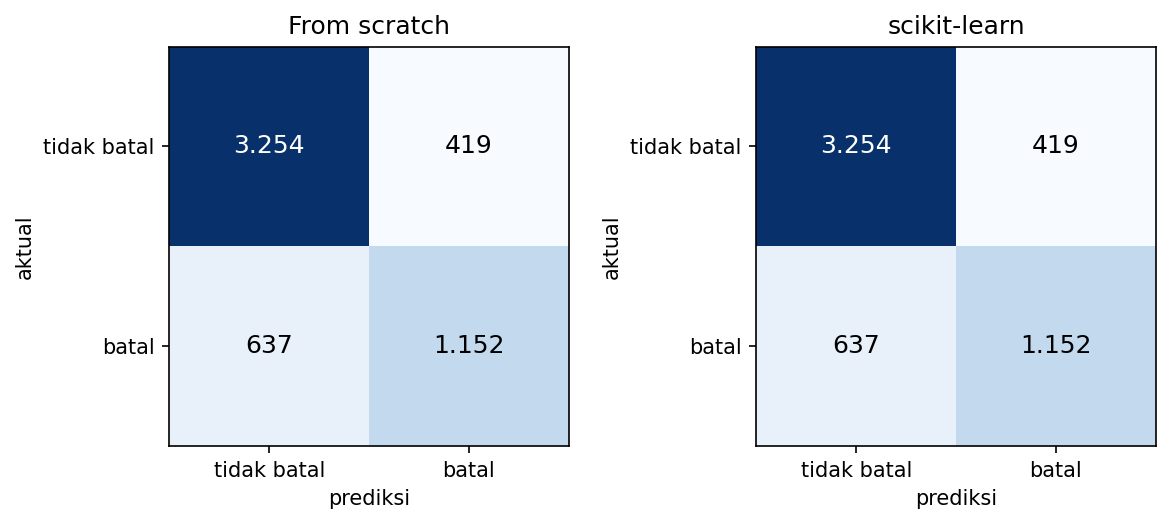
\includegraphics[width=0.8\textwidth]{lr/lr_confusion_matrix.png}
	\caption{\textit{Confusion matrix} LR tanpa penalti (konfigurasi terbaik) pada \texttt{val\_set}, \textit{from scratch} (kiri) dan \textit{scikit-learn} (kanan)}
	\label{fig:lr-cm}
\end{figure}

\subsubsection{Kurva \textit{Loss}}
Gambar~\ref{fig:lr-loss} memperlihatkan nilai fungsi tujuan $J$ (\textit{log-loss} ditambah penalti) pada \texttt{train\_set} untuk setiap penalti, dengan kedua \textit{solver} yang diimplementasikan. Nilai $J$ tidak dapat dibandingkan langsung antarpenalti karena suku penaltinya berbeda; yang dibandingkan adalah bentuk konvergensinya.

\begin{figure}[H]
	\centering
	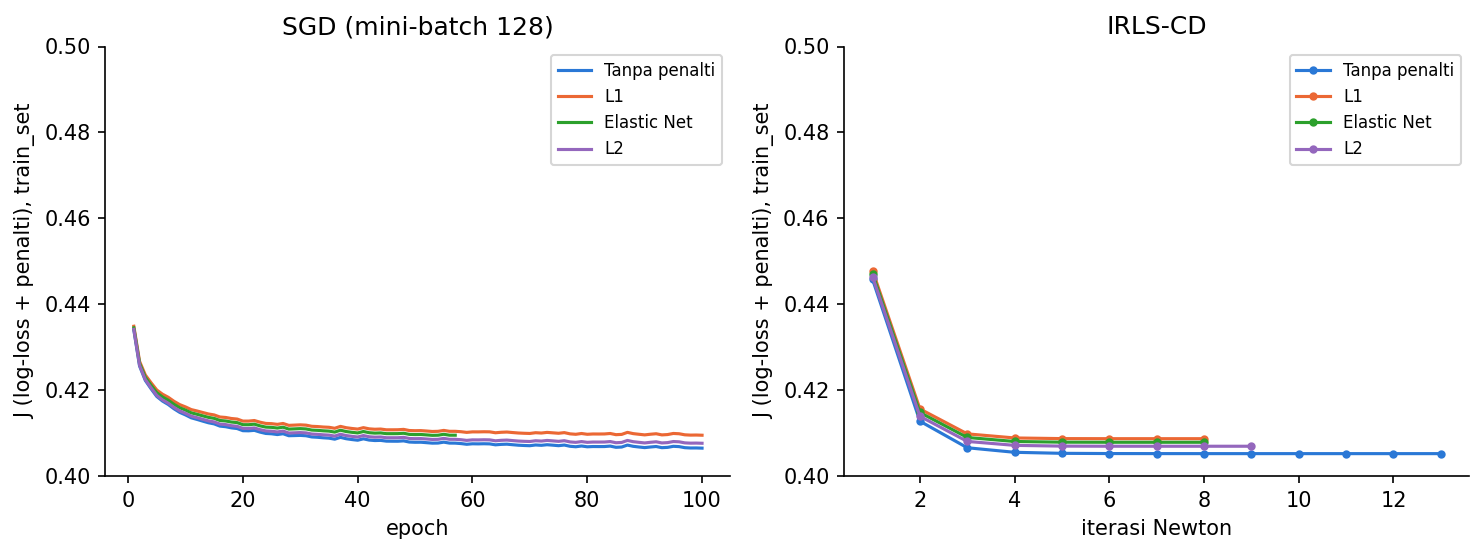
\includegraphics[width=\textwidth]{lr/lr_loss_curves.png}
	\caption{Kurva $J$ per iterasi pada \texttt{train\_set}: SGD \textit{mini-batch} per \textit{epoch} (kiri) dan IRLS-CD per iterasi Newton (kanan)}
	\label{fig:lr-loss}
\end{figure}

\begin{itemize}
	\item \textbf{SGD} menurun cepat pada sekitar 10 \textit{epoch} pertama, lalu melandai dan masih turun perlahan saat berhenti. Tiga dari empat konfigurasi berhenti di batas 100 \textit{epoch}; hanya \textit{Elastic Net} berhenti lebih awal (57 \textit{epoch}) karena perubahan \textit{loss} di bawah toleransi. Kurvanya sedikit bergerigi karena gradien \textit{mini-batch} bersifat acak, dan \textit{learning rate} yang tetap membuatnya tidak pernah menetap di satu titik. Ini berarti SGD belum benar-benar konvergen pada 100 \textit{epoch}.
	\item \textbf{IRLS-CD} mencapai nilai akhirnya dalam 8 sampai 13 iterasi. Pada tanpa penalti dibutuhkan 13 iterasi, lebih banyak daripada penalti lain (8 sampai 9), karena tidak ada suku penalti yang membuat masalah lebih terkondisi dengan baik; model ini juga memiliki kolom yang kolinear (Subbab~\ref{subsec:lr-implementasi}).
	\item Untuk setiap penalti, $J$ akhir IRLS-CD lebih rendah daripada SGD: 0,4052 terhadap 0,4065 (tanpa penalti), 0,4087 terhadap 0,4095 (L1), 0,4079 terhadap 0,4095 (\textit{Elastic Net}), dan 0,4070 terhadap 0,4076 (L2). Karena fungsi tujuannya konveks, selisih ini adalah jarak SGD ke optimum, yang menjelaskan mengapa IRLS-CD sedikit lebih baik pada validasi (Subbab~\ref{subsubsec:lr-optimasi}).
\end{itemize}

\subsubsection{Analisis}
\paragraph{Hasil praktis identik.} Untuk keempat penalti, selisih Macro F1 antara \textit{scratch} dan \textit{scikit-learn} paling besar 0,0003 (L1), ROC-AUC berselisih paling besar $10^{-4}$, dan matriks konfusinya sama persis atau berbeda satu baris. Label prediksi sama pada 99,98\% sampai 100\% baris, dan korelasi peluang model terbaik 1,0000. Ini sesuai harapan: keduanya meminimumkan fungsi tujuan konveks yang sama, sehingga IRLS-CD dan \textit{solver} \textit{scikit-learn} menuju optimum yang sama. Perbedaan kecil pada L1 berasal dari kriteria berhenti yang berbeda: \texttt{saga} berhenti pada toleransi tertentu dan belum tentu tepat di optimum, sedangkan IRLS-CD pada L1 menghasilkan nilai $J$ sedikit lebih rendah (0,408706 terhadap 0,408709).

\paragraph{Bobot dan \textit{sparsity}.} Selisih bobot terbesar (nilai mutlak) antara kedua implementasi adalah 5,85 (tanpa penalti), 0,100 (L1), 0,062 (\textit{Elastic Net}), dan 0,0028 (L2). Selisih besar pada model tanpa penalti bukan tanda kesalahan. Kolom \textit{one-hot} setiap fitur kategorikal bersama bias saling kolinear (matriks fitur ditambah bias hanya berperingkat 92 dari 101), sehingga bobotnya tidak unik walaupun prediksinya identik (label sama 100\%). Penalti L2 memperbaiki hal ini karena menjamin solusi yang unik, dan itu terlihat dari selisih bobotnya yang sangat kecil. Pada L1 dan \textit{Elastic Net}, kedua implementasi menghasilkan bobot tepat nol dalam jumlah hampir sama (16 terhadap 14 dan 13 terhadap 12). Selisih satu sampai dua bobot muncul karena bobot-bobot itu berada tepat di dekat ambang \textit{soft-thresholding}, dan kriteria berhenti kedua \textit{solver} berbeda.

\paragraph{Waktu pelatihan.} Waktu pada Tabel~\ref{tab:lr-hasil} hanya perkiraan kasar karena diukur sekali pada komputer yang sedang dipakai untuk pekerjaan lain. Pengulangan pengukuran yang sama memberi angka yang berbeda beberapa kali lipat (misalnya \textit{scikit-learn} tanpa penalti: 10,9 detik pada satu kali jalan dan 35,8 detik pada kali lain), sehingga hanya selisih yang besar yang bermakna. Terlihat dua pola. \textit{Scikit-learn} jauh lebih cepat pada L2 (2,2 terhadap 13,1 detik), karena \texttt{lbfgs} yang ditulis dalam kode teroptimasi hanya perlu menghitung gradien, sedangkan IRLS-CD membentuk dan memperbarui matriks Gram $101 \times 101$ pada setiap iterasi. Sebaliknya \textit{scratch} jauh lebih cepat pada L1 dan \textit{Elastic Net} (sekitar 9 sampai 11 detik terhadap lebih dari 360 detik), karena \texttt{saga} adalah metode orde pertama yang butuh banyak lintasan data sampai mencapai toleransi $10^{-6}$ pada fitur yang berkorelasi, sedangkan IRLS-CD memakai informasi orde kedua dan konvergen dalam kurang dari sepuluh iterasi. Pada model tanpa penalti \textit{scratch} juga lebih cepat (7,5 terhadap 35,8 detik), tetapi selisih ini paling tidak stabil antarpengukuran. Perbandingan ini adil hanya dalam arti kedua \textit{solver} diminta ketat pada toleransi masing-masing; \textit{scikit-learn} dapat dipercepat dengan toleransi yang lebih longgar tanpa mengubah hasil prediksi secara berarti.

\paragraph{Keterbatasan.} (i) Perbandingan dilakukan pada satu pembagian \texttt{train\_set}/\allowbreak\texttt{val\_set}, dan \texttt{val\_set} ikut dipakai dalam CV sehingga bukan estimasi independen (Subbab~\ref{subsec:lr-validasi}). (ii) Selisih antarpenalti (paling besar 0,002 pada Macro F1) jauh di bawah simpangan baku antar-\textit{fold} (0,0073), sehingga urutan penalti pada tabel tidak bermakna secara statistik. (iii) Seluruh hasil \textit{scratch} di atas memakai IRLS-CD. Hasil \textit{scratch} dengan \textit{solver} SGD yang sesuai materi kelas sedikit di bawahnya (Subbab~\ref{subsubsec:lr-optimasi}); karena SGD belum konvergen, selisihnya dengan \textit{scikit-learn} akan lebih besar dari angka di atas.

\subsection{Bonus LR}
\label{subsec:lr-bonus}

\todo{Hapus subbab bonus yang tidak dikerjakan.}

\subsubsection{Video Kontur \textit{Log-Loss}}
\todo{Video kontur \textit{log-loss} pada bidang $(\theta_0, \theta_1)$ beserta lintasan parameter selama pelatihan. Jelaskan cara pembuatannya, cantumkan cuplikan \textit{frame}, dan tautan atau lokasi berkas video.}

\begin{figure}[H]
	\centering
	\placeholdergambar{Video Kontur \textit{Log-Loss}}
	\caption{Video Kontur \textit{Log-Loss} LR}
	\label{fig:lr-bonus-0}
\end{figure}

\subsubsection{Algoritma Optimasi di Luar Materi Kelas}
\todo{Jika ada: jelaskan algoritmanya, mengapa dapat mengoptimasi model, bukti perbaikannya (sebelum vs sesudah), dan \textbf{referensinya (tanpa referensi bonus dianulir)}. Misalnya \textit{mini-batch} SGD dengan \textit{early stopping}, \textit{momentum}, Adam, atau \textit{proximal gradient} untuk L1.}

